\documentclass{article}
\usepackage[margin=2cm]{geometry}
\usepackage{graphicx}
\usepackage{float}
\usepackage{booktabs}
\usepackage{hyperref}
\usepackage{titlesec}
\titlespacing*{\section}{0pt}{2ex plus 0.5ex minus 0.2ex}{1ex plus 0.2ex}
\titlespacing*{\subsection}{0pt}{1.5ex plus 0.3ex minus 0.2ex}{0.6ex plus 0.1ex}
 
\setlength{\intextsep}{6pt plus 2pt minus 2pt}
\setlength{\textfloatsep}{8pt plus 2pt minus 4pt}
\setlength{\abovecaptionskip}{4pt}
 
\title{Diabetes Risk Factors: A Correlation Analysis of Lifestyle and Biological Variables}
\author{Ilan Noè van Woerden (i6352457)}
\date{October 2026}
 
\begin{document}
 
\begin{titlepage}
  \vspace*{\fill}
  \begin{center}
    {\LARGE\bfseries Diabetes Risk Factors:\\[1ex]
     A Correlation Analysis of Lifestyle\\and Biological Variables\par}
  \end{center}
  \vspace*{\fill}
  \begin{flushright}
    Ilan Noè van Woerden (i6352457)\\
    Introduction to Programming (MAT2007)\\
    Maastricht University\\
    Coordinator: Panos Christakoglou\\
    October 2026
  \end{flushright}
\end{titlepage}

\section{Introduction}
Diabetes is one of the most prevalent chronic diseases in the world~\cite{who}, and identifying which risk factors matter most helps to prevent it. Some risk factors are behaviours that a person can change, such as diet, physical activity, smoking and alcohol consumption. Others are biological characteristics, namely age, family history and BMI. This differentiation matters, because, if lifestyle dominates, programmes that aim to improve lifestyle should work, whereas if biology dominates, being able to identify high-risk people early matters more.

This report aims to answer: \textbf{do lifestyle factors predict diabetes risk as strongly as fixed biological factors?} Lifestyle variables (exercise hours, daily walking, sleep, diet quality, smoking, and alcohol consumption) are compared against biological variables (age, BMI, family history) using their correlation with a patient's diabetes risk score. Each variable is examined individually, and the two groups are compared on average. It is hypothesised that lifestyle factors correlate with risk at least as strongly as biological factors.

\section{Methods}
\subsection{Dataset}
A synthetic patient health dataset is used from Kaggle~\cite{dataset} with 50,000 patients and 41 variables that cover demographics, biometrics, lifestyle habits and existing conditions. The outcome is \texttt{Diabetes\_Risk\_Score}, which ranges from 13 to 100 and has no missing values. Furthermore, at most 4\% of the values of any variable used are missing (sleep hours), so no rows were removed. Each correlation uses the patients with complete data for that pair of variables. Ordered categories (diet quality, smoking, alcohol) were encoded as 1, 2, 3, and family history as 0, 1.  

\subsection{Statistical analysis}
For each predictor, the Pearson correlation coefficient~\cite{pearson} $r$ with the risk score was computed. This measures the strength and direction of their linear relationship, and ranges from $-1$ to $1$. To test whether a correlation differs from zero ($H_0:\rho=0$) the following test statistic was used:
\begin{equation}
  t = \frac{r\sqrt{N-2}}{\sqrt{1-r^{2}}},
\end{equation}
where $N$ is the number of patients with complete data for the pair of variables. Under $H_0$, $t$ follows a Student's $t$ distribution with $N-2$ degrees of freedom. With $N\approx50,000$, the standard error of each $r$ is around $0.004$. The coefficient of determination ($r^2$) is also computed, which is the share of the variation in the risk score explained by that variable alone.

The two groups (six lifestyle and three biological variables) were then compared through their mean absolute correlation, $\langle |r|\rangle$,  which is the average of $|r|$ over the variables in each group. Note that this is only a descriptive comparison, not a test. The analysis was done in R and the plots produced in Python (code is available on GitHub\footnote{\url{https://github.com/ilannvw/Diabetes-Risk}}).

\section{Results}
Table~\ref{tab:corr} and Figure~\ref{fig:both} show the  correlation of every variable with the risk score. The three biological factors rank highest, namely: family history ($r=0.308$), age ($r=0.279$) and BMI ($r=0.226$). The strongest lifestyle factor is diet quality ($r=-0.154$), then smoking ($r=0.131$) and alcohol ($r=0.104$). All of these correlations, and sleep hours ($r=-0.075$), differ significantly from zero ($p<0.001$). However, exercise hours ($t=-0.45$, $p=0.65$) and daily walking ($t=-0.16$, $p=0.87$) are the exceptions, as they are essentially uncorrelated with risk ($|r|<0.003$). On average, biological factors are about 3.5 times more correlated with the risk score ($\langle|r|\rangle=0.271$) than lifestyle factors ($\langle|r|\rangle=0.078$).

Family history alone explains about 9.5\% of the variation in the risk score, age 7.8\% and BMI 5.1\%, whereas the best lifestyle predictor, diet quality, explains only 2.4\%. Figure~\ref{fig:both} (right) illustrates the strongest predictor: patients with a family history of diabetes have a clearly higher median risk score (80) than those without (70), and a higher mean (78.9 against 69.3).

\begin{table}[ht]
  \centering
  \footnotesize
  \caption{Correlation ($r$), variance explained ($r^2$) and $t$-test against zero for each variable (df between 47{,}981 and 49{,}998).}
  \label{tab:corr}
  \begin{tabular}{llrrrr}
    \toprule
    Variable & Group & $r$ & $r^2$ & $t$ & $p$ \\
    \midrule
    Family history & Biological & $0.308$ & $0.095$ & $72.3$ & $<0.001$ \\
    Age & Biological & $0.279$ & $0.078$ & $64.6$ & $<0.001$ \\
    BMI & Biological & $0.226$ & $0.051$ & $51.8$ & $<0.001$ \\
    Diet quality & Lifestyle & $-0.154$ & $0.024$ & $-34.9$ & $<0.001$ \\
    Smoking & Lifestyle & $0.131$ & $0.017$ & $29.5$ & $<0.001$ \\
    Alcohol & Lifestyle & $0.104$ & $0.011$ & $23.5$ & $<0.001$ \\
    Sleep hours & Lifestyle & $-0.075$ & $0.006$ & $-16.4$ & $<0.001$ \\
    Exercise hours & Lifestyle & $-0.002$ & $<0.001$ & $-0.45$ & $0.65$ \\
    Daily walking & Lifestyle & $-0.001$ & $<0.001$ & $-0.16$ & $0.87$ \\
    \bottomrule
  \end{tabular}
\end{table}

\begin{figure}[H]
  \centering
  \begin{minipage}[t]{0.44\linewidth}
    \centering
    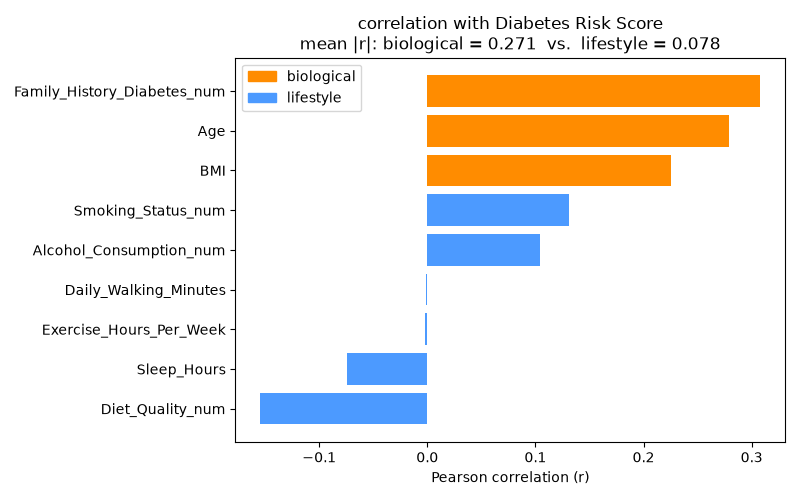
\includegraphics[width=\linewidth]{correlation_comparison.png}
  \end{minipage}\hfill
  \begin{minipage}[t]{0.32\linewidth}
    \centering
    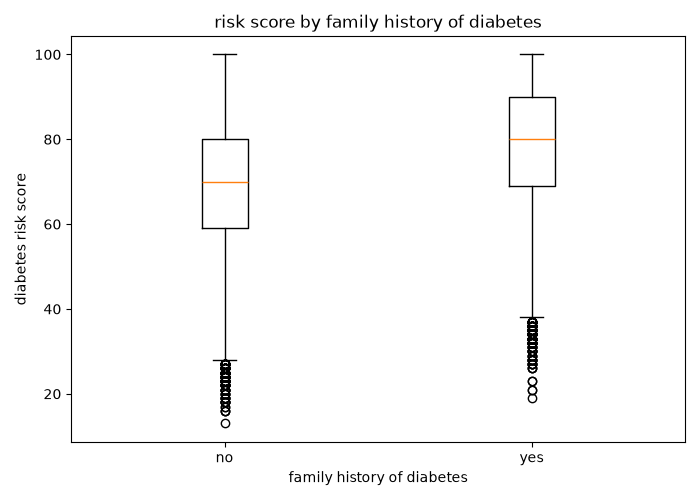
\includegraphics[width=\linewidth]{risk_by_family_history.png}
  \end{minipage}
  \caption{Left: Pearson correlation of each variable with the diabetes risk score, coloured by group. Right: diabetes risk score by family history of diabetes.}
  \label{fig:both}
\end{figure}

\section{Discussion}
The results show a clear hierarchy; the three biological variables are more strongly associated with the risk score than any lifestyle variable. The most surprising result is that exercise hours and daily walking are uncorrelated with risk. This would be unexpected in actual clinical data, where a lifestyle programme including regular physical activity reduced the incidence of type 2 diabetes by 58\% in high-risk adults~\cite{knowler}. This may indicate that the synthetic risk score was not generated with these variables in mind. Because the sample is so large (50,000 patients), even very weak correlations are statistically significant; sleep hours ($r^2=0.006$) and family history ($r^2=0.095$) both have $p<0.001$. The $p$-value only indicates whether a correlation differs from zero ($H_0:\rho=0$), whereas $r$ and $r^2$ quantify its strength and how much of the differences in risk scores it accounts for. Effect size is therefore more informative here than significance.

Several limitations should be taken into account. Correlation does not imply causation, as two variables can be linked without one causing the other. The data are synthetic, so the findings do not describe real-life patients. Pearson correlation only captures linear relationships, and by categorising the variables, it assumes 1, 2, and 3 are equally spaced. Moreover, the split into groups is not completely clean, since in real populations BMI is influenced by diet and exercise, but in this dataset, the predictors are almost uncorrelated with each other (e.g.\ BMI with diet quality gives $r=-0.006$).

\section{Conclusion}

In this dataset, biological factors are on average about $3.5\times$ more strongly correlated with diabetes risk than lifestyle factors ($\langle|r|\rangle=0.271$ against $0.078$), and family history is the strongest single predictor. As the data are synthetic, these conclusions describe the dataset, not real patients. 
{\footnotesize
\setlength{\itemsep}{0pt}\setlength{\parskip}{0pt}
\begin{thebibliography}{9}
\bibitem{who} World Health Organization. Diabetes [Fact sheet].
\url{https://www.who.int/news-room/fact-sheets/detail/diabetes}
\bibitem{dataset} Diabetes Risk Prediction Dataset, Kaggle.
\url{https://www.kaggle.com/datasets/srisyra02/diabetes-risk-prediction-dataset}
\bibitem{pearson} Pearson, K. (1895). Notes on regression and inheritance in the case of two parents. \textit{Proceedings of the Royal Society of London}, 58, 240--242.
\url{https://doi.org/10.1098/rspl.1895.0041}
\bibitem{knowler} Knowler, W. C., et al. (2002). Reduction in the incidence of type 2 diabetes with lifestyle intervention or metformin. \textit{New England Journal of Medicine}, 346(6), 393--403.
\url{https://doi.org/10.1056/NEJMoa012512}
\end{thebibliography}
}

\end{document}